\documentclass[../Analysis-3]{subfiles}

\begin{document}
\chapter*{Lecture 28} %Set chapter name
\addcontentsline{toc}{chapter}{Lecture 28} %Set chapter title
\setcounter{chapter}{28} %Set chapter counter
\setcounter{section}{0}

\newcommand{\inti}[3]{\int_{#1} {#2} \hspace{0.1cm} \dd {#3}}
%The content

\section{Green's Theorem}
\begin{Thm}{$\R^2$ version of Green's Theorem}{gtm}
    Let $\mathcal{R} \subseteq \R^2 $ be a simply connected domain with boundary curve $\mathcal{C}$ where parametrization is taken in anti-clockwise direction. Let $\vec{F} = (P,Q)$ be a $C^1$ vector field on $\mathcal{R}$, then
    \[
        \int_{\mathcal{C}} \vec{F} \cdot \dd r := \int_{\mathcal{C}} P \, \dd x + Q \, \dd y = \int_{\mathcal{R}} \left( \pdv{Q}{x} - \pdv{P}{y}\right) \dd A
    \]
\end{Thm}

\begin{proofFig}{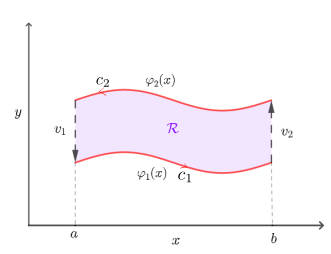
\includegraphics[width=.78\linewidth]{../figures/lec-28.1.png}}{A simple region} (for Simple region)

    Let, $\mathcal{R} = \qty{(x,y) | a\le x\le b, \varphi_1(x) \le y \le \varphi_2(x)}$ be a simple region. Here $\mathcal{C} = \mathcal{C}_1 \cup v_2 \cup \mathcal{C}_2 \cup v_1$ is the curve bounding the region along anti-clockwise direction (as shown in the picture).

    \begin{align*}
        -\int_{\mathcal{R}} \pdv{P}{y} \dd A & = -\int_{a}^{b} \int_{\varphi_1(x)}^{\varphi_2(x)} \pdv{P}{y} \dd y \dd x \\
                                             & = - \int_{a}^{b} (P(x,\varphi_2(x))-P(x,\varphi_1(x))) \dd x              \\
    \end{align*}

    Now, $\mathcal{C}_1,\mathcal{C}_2,v_1,v_2$ can be explicitly written as,
    \begin{align*}
        v_1           & = \qty{(a,t) | \varphi_1(a) \le t \le \varphi_2(a)} \\
        \mathcal{C}_1 & = \qty{(x,\varphi_1(x)) | a \le x \le b}            \\
        v_2           & = \qty{(a,t) | \varphi_1(b) \le t \le \varphi_2(b)} \\
        \mathcal{C}_2 & = \qty{(x,\varphi_2(x)) | a \le x \le b}
    \end{align*}

    Now,

    \begin{align*}
        \int_{v_1} P \dd x                 & = \int_{v_1} P(x(t),y(t)) \dv{x(t)}{t} \dd t = 0 \\
        \int_{\mathcal{C}_1} P \dd x       & = \int_{a}^{b} P(t,\varphi_1(t)) \dd t           \\
        \int_{\mathcal{C}_2} P \dd x       & = \int_{a}^{b} P(t,\varphi_2(t)) \dd t           \\
        \implies \int_{\mathcal{C}} P\dd x & = -\int_{\mathcal{R}} \pdv{P}{y} \dd A
    \end{align*}


    By similar mechanism we can show $\displaystyle\int_{\mathcal{C}} Q \dd y = \int_{\mathcal{R}} \pdv{Q}{y} \dd A$. The rest follows from here.
\end{proofFig}

\begin{Eg}{}{}
    Let, $\mathcal{C}$ be the boundary of $[0,1]^2$, i.e., $\partial [0,1]\times[0,1] = \mathcal{C}$. Evaluate

    \[\int_{\mathcal{C}} \langle x^2-y^2,2xy \rangle\]
    \textit{Solution.} We can decompose $\mathcal{C} = \mathcal{C}_1 \cup \mathcal{C}_2 \cup \mathcal{C}_3 \cup \mathcal{C}_4$ (as in the following picture)

    \begin{wrapfigure}{r}{0.25\textwidth}
        \centering
        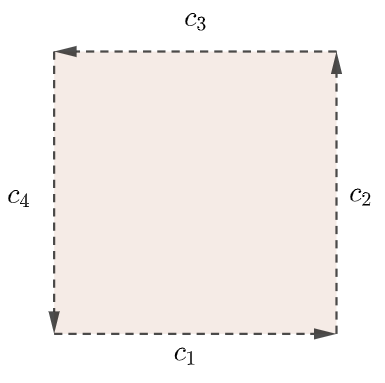
\includegraphics[width=.78\linewidth]{../figures/lec-28.2.png}
        \caption{$\partial( [0,1]^2)$}
    \end{wrapfigure}

    Let, $P(x,y) = x^2 - y^2, Q(x,y) = 2xy$. Then the integral,

    \begin{align*}
        \int_{\mathcal{C}} P \dd x + Q \dd y & = \iint_{[0,1]^2} (2y + 2y) \dd A \hspace{0.2cm} \text{(Green's Theorem)} \\
                                             & = \int_{0}^1 \int_0^1 4y \hspace{0.1cm} \dd y \dd x                       \\
                                             & = 2
    \end{align*}

    If we try to calculate the integral \textbf{directly}, we will end up getting same result.

    $\hfill \blacksquare$
\end{Eg}

\begin{tcolorbox}
    \textbf{Area of a closed Region.} Let, $\mathcal{R}$(simply connected) be a closed region and $\mathcal{C} = \partial{\mathcal{R}}$ be the curve enclosing the region. Using Green's Theorem we get,

    \[\Area(\mathcal{R}) = \int_{\mathcal{R}} \dd A = \int_{\mathcal{C}} x \dd y = \int_{\mathcal{C}} -y \dd x = \int_{\mathcal{C}} \frac{x \dd y -y \dd x}{2} \]

\end{tcolorbox}

\begin{Eg}{Area inside the ellipse: $\frac{x^2}{a^2} + \frac{y^2}{b^2} = 1$}{}

    \textit{Solution.} Parametrization of ellipse $x = a \cos t, y = b \sin t$ where $t \in [0,2\pi)$. Using the above application of Green's Theorem we can write,
    \[\Area = \int_{\mathcal{C}} x \dd y = ab \int_{0}^{2\pi} \cos^2t \dd t = \pi ab \]
    $\hfill \blacksquare$
\end{Eg}

\begin{Thm}{Independence of path}{}
    Let $\vec{F}$ be a $C^1$ vector field on $\R^2$ such that $\displaystyle\int_{\mathcal{C}} \vec{F} \cdot \dd \vec{r}$ is independent of path. Then $\vec{F}$ is conservative over an open and simply connected domain.
\end{Thm}

\begin{proof}
    Let, $\mathcal{D}$ be an open and connected domain. $\vec{F} = \inp{P}{Q}$ is defined over $\mathcal{D}$. Also let, $P_0 = \inp{x_0}{y_0}$ be a fixed point in the domain $\mathcal{D}$ and $P_1 = \inp{x}{y} \in \mathcal{D}$ be a variable point. $\mathcal{C}$ be a smooth curve joining $P_0$ and $P_1$. Define

    \[\varphi(x,y) = \inti{\mathcal{C}}{\vec{F} \cdot }{\vec{r}}\]

    Since, $\mathcal{D}$ is open set, so we must get an open ball centered at $P_1$ contained in $\mathcal{D}$. Take a point $P_1'= \inp{x_1}{y}$ inside that open ball such that $x_1 < x$. Let, $\mathcal{C}_1$ be a  smooth curve from $P_0$ to $P_1$ and $\mathcal{C}_2$ be a line segment from $P_1'$ to $P_1$. So, $\mathcal{C}_1 \cup \mathcal{C}_2$ defines a smooth curve from $P_0$ to $P_1$.

    \[\begin{tikzcd}
            && {P_1'(x_1,y)} && {P_1(x,y)} \\
            \\
            {P_0(x_0,y_0)}
            \arrow["{\mathcal{C}_1}", curve={height=-18pt}, from=3-1, to=1-3]
            \arrow["{\mathcal{C}_2}", from=1-3, to=1-5]
            \arrow["{\mathcal{C}}"', curve={height=18pt}, from=3-1, to=1-5]
        \end{tikzcd}\]

    As $\displaystyle\inti{\mathcal{C}}{\vec{F} \cdot }{\vec{r}}$ is path independent We can write, \[
        \varphi(x,y) = \inti{\mathcal{C}_1}{\vec{F} \cdot }{\vec{r}} + \inti{\mathcal{C}_2}{\vec{F} \cdot }{\vec{r}}
    \]

    Now we take the partial derivative of both sides of this equation with respect to $x$. The first integral does not depend on the variable $x$ since $\mathcal{C}_1$ is the path from $P_0(x_0,y_0,z_0)$ to $P'_1(x_1,y,z)$ and so partial differentiating this line integral with respect to $x$ is zero.

    \begin{align*}
        \pdv{\varphi}{x} & =\pdv{x} \left( \inti{\mathcal{C}_1}{\vec{F} \cdot }{\vec{r}} + \inti{\mathcal{C}_2}{\vec{F} \cdot }{\vec{r}} \right)                                           \\
                         & = \underbrace{\pdv{x} \left( \inti{\mathcal{C}_1}{\vec{F} \cdot }{\vec{r}}\right)}_{= 0}  + \pdv{x} \left(\inti{\mathcal{C}_2}{\vec{F} \cdot }{\vec{r}} \right)
    \end{align*}

    Now,$\mathcal{C}_2$ can be parametrized as $r(t) = \inp{t}{y}$ where $t \in [x_1,x]$. So,

    \begin{align*}
        \pdv{x} \left(\inti{\mathcal{C}_2}{\vec{F} \cdot }{\vec{r}}\right) & = \pdv{x} \left( \int_{x_1}^x \inp{P(t,y)}{Q(t,y)} \cdot \inp{1}{0} \dd{t} \right) \\
                                                                           & = \pdv{x} \left( \int_{x_1}^x P(t,y) \dd{t} \right)                                \\
                                                                           & = P(x,y) \hspace{0.2cm} \text{[Fundamental Theorem of calculus]}
    \end{align*}

    Similarly, we can show that, $\pdv{\varphi}{y} = Q(x,y)$. And hence, $\grad\varphi = \vec{F}(x,y)$. We can define $\varphi$ as the potential of $\vec{F}$.
\end{proof}

\begin{Thm}{}{}
    Let, $\mathcal{D}$ be a simply connected domain in $\R^2$ and $\vec{F}$ is a $C^1$ vector field on $\mathcal{D}$. Then $\vec{F}$ is conservative iff $\curl \vec{F} = 0$ on $\mathcal{D}$.
\end{Thm}

\begin{proof}
    ($\Rightarrow$) This direction is trivial.

    \

    ($\Leftarrow$) From Green's Theorem we can say that $ \displaystyle\inti{\mathcal{C}}{\vec{F} \cdot }{\vec{r}} = 0$ over all closed curve $\mathcal{C}$. For any two point $p_0,p_1 \in \mathcal{D}$ if $\gamma_1, \gamma_2 : [0,1] \to \mathcal{D}$ are two smooth curves joining $p_0$ and $p_1$. (i.e., $\gamma_1(0) = \gamma_2 (0) = p_0$ and $\gamma_1(1) = \gamma_2(1) = p_1$) then $\gamma_1 \cup \gamma_2(1-t)$ is a closed curve. So, $ \displaystyle\inti{\gamma_1}{\vec{F} \cdot }{\vec{r}}  = \displaystyle\inti{\gamma_2}{\vec{F} \cdot }{\vec{r}}$. Which means the integral is path independent. Using the previous theorem we can say, $\vec{F}$ is conservative on $\mathcal{D}$.
\end{proof}

\section{Gauss Divergence Theorem}

\begin{Def}{Divergence of a vector field}{}
    \small  Given a vector field $\vec{F} = (f_1,\cdots, f_n) : \R^n \to \R^n $, the ``Divergence'' of $\vec{F}$ is,

    \[\text{div}(F) = \sum_{i=1}^{n} \pdv{f_i}{x_i} \equiv \div \vec{F}\]
\end{Def}

\begin{Thm}{Gauss Divergence Theorem}{gdt}
    Let, $\mathcal{D} \subseteq \R^3$ a solid domain, $\partial{\mathcal{D}}$ be an oriented surface. Let,  $\vec{F} = \inp{P}{Q,R}$ be a $C^1$ vector field on an open surface containing $\mathcal{D} \cup \partial{\mathcal{D}}$. Then,
    \[
        \underbrace{\inti{\partial{\mathcal{D}} = \mathcal{S}}{\vec{F}\cdot}{\vec{S}}}_\text{surface integral} = \underbrace{\inti{\mathcal{D}}{\div \vec{F}}{V}}_\text{volume integral}
    \]
\end{Thm}

Just like FTC, the behavior over a volume is fully determined by the behavior at the boundary. Proof of this theorem is beyond our reach. But we can see the proof for simple cases.

\vspace{0.2cm}

\begin{proof}
    (For a simple case) Consider $\mathcal{D} = \qty{(x,y,z) | \varphi_1(x,y) \le z \le \varphi_2(x,y), (x,y) \in [a,b]\times [c,d]}$.

    (\textbf{Exercise.}) Complete the proof!
\end{proof}

%%%%%%%%%%%%%%%%%%%%%%


\begin{Eg}{}{}
    $F (x,y,z) = \inp{x+y}{z^2,x^2}$ and $S$ be the hemisphere $x^2+y^2+z^2 = 1, z>0$. Compute,
    \[\int_{S} \vec{F} \dd \vec{S}\]

    \textit{Solution.} Notice that $S$ is open surface. We want to  use Gauss Theorem ($\ref{th:gdt}$) so we need a close surface. Let, $S_1$ be the surface $x^2 +y^2 \le 1$. Then $S \sqcup S_1$ is a closed surface.

    \begin{align*}
        \int_{S \sqcup S_1} \vec{F}\cdot \dd \vec{S} & = \int_{x^2+y^2,z^2 \le 1, z \ge 0} \div \vec{F} \dd{V} \\
                                                     & = \int_{x^2+y^2,z^2 \le 1, z \ge 0}\,\dd{V}           \\
                                                     & = \frac{2\pi}{3}
    \end{align*}

    Parametrization of the surface $S_1 =\qty{(x,y,0) | x^2+y^2 = 1}$. So, $r_x \times r_y = \inp{1,0}{0} \times \inp{0,1}{0}$.

    \begin{align*}
        \int_{S_1} \vec{F} \cdot \dd \vec{S}           & = \int_{x^2+y^2 \le 1} \inp{x+y}{z^2,x^2} \cdot \inp{0,0}{1} \dd{A} = \int_{x^2+y^2 \le 1} x^2 \dd{A} \\
                                                       & = \int_{0}^{2\pi} \int_{0}^{1} r^3 \cos^2 \theta \,dr \,d\theta = \frac{\pi}{4}                       \\
        \Rightarrow \int_{S} \vec{F} \cdot \dd \vec{S} & = \frac{11\pi}{12}
    \end{align*}
\end{Eg}

\section{Stokes' Theorem}
\begin{Thm}{Stokes' Theorem}{st}
    Let, $\mathcal{C}$ be a $C^1$ curve enclosing an oriented surface $\mathcal{S}$ in $\R^3$. Let,  $\vec{F} = \inp{P,Q}{R}$ be a $C^1$ vector field on an open set containing $\mathcal{S}$. Then,

    \small \[\inti{\mathcal{C}}{\vec{F} \cdot }{\vec{r}} = \inti{\mathcal{S}}{(\curl \vec{F}) \cdot}{\vec{S}}  \]

    $\bullet$ Here orientation of $\mathcal{S}$ and direction of $\mathcal{C}$ is same.
\end{Thm}

\begin{Eg}{}{}
    Compute $\displaystyle\inti{\mathcal{C}}{\vec{F} \cdot }{\vec{r}}$, where $\mathcal{C} : x^2 +y^2 = 9, z =4$ and $\vec{F} = \inp{-y,x}{xyz}$.

    \textit{Solution.} $\curl \vec{F} = \inp{xz,-yz,}{2}$. By convention, we should assume direction of $\mathcal{C}$ is along counter-clockwise direction. So,  The normal vector of $\mathcal{S}$ is along -ve $z$ axis. So, required integral,

    \begin{align*}
        \inti{\mathcal{C}}{\vec{F} \cdot }{\vec{r}} & = \inti{\mathcal{S}}{(\curl \vec{F}) \cdot}{\vec{S}}                     \\
                                                    & = \int_{x^2+y^2 \le 1, z =4 } (\curl \vec{F}) \cdot \inp{0,0}{-1} \dd{A} \\
                                                    & = -2 \int_{x^2+y^2 \le 1, z =4} \dd{A}                                   \\
                                                    & = -18\pi
    \end{align*}

\end{Eg}


Stoke's Theorem is $\R^3-$analogue of Green's Theorem ($\ref{th:gtm}$). If we take the third component of $\vec{F}$ as zero, i.e., $R =0$ then Stoke's Theorem ($\ref{th:st}$) gives us back Green's Theorem ($\ref{th:gtm}$).

\begin{tcolorbox}
    There is a generalized version of stokes theorem. Just for information the theorem is stated below.

    $\bullet$ If $\Omega$ is an oriented $n$-manifold (with boundary) and $\omega$ is a differential form ($(n-1)$ form). Then integral of $\omega$ over the boundary $\partial \Omega$ of the manifold $\Omega$ is given by,

    \[\int_{\partial \Omega} \omega = \int_{\Omega} \dd \omega\]

\end{tcolorbox}

\end{document}
